\begingroup
\RaggedRight

\begin{quote}
"On what is fear: non-acceptance of uncertainty. If we accept that uncertainty it becomes an adventure!"
\newline
\hfill  — \textit{Jalāl al-Dīn Muḥammad Rūmī}
\end{quote}

\section*{Introduction}
Hardware Trojan (HT) insertion has become a major concern in today's fabless semiconductor manufacturing since attackers can make malicious modifications for a variety of reasons, such as information leakage, incorrect operation, or inflicting damage on the chip \cite{salmani2017hardware, Regazzoni:HTDetection, Guin:HTDetection, Salmani:HTDetection}. The possibility of HTs being inserted at different manufacturing stages increases, presenting a significant security threat to hardware systems. Vulnerabilities range from RTL code and third-party IP integration in the design phase to potential insertions during EDA processes like synthesis, optimization, and place-and-route. Mask preparation \cite{belous2020methods} and lithography in wafer fabrication offer additional points of vulnerability. Packaging and testing phases also present opportunities for Trojan inclusion, as do third-party manufacturing and distribution in post-production. Robust security measures \cite{narasimhan2011tesr}, including hardware design practices \cite{muralidhar2021contrastive}, supply chain management \cite{chang2023supplier, panduro2023effective}, and thorough post-manufacturing testing \cite{monjur2023hardware}, are imperative to mitigate these risks in the semiconductor industry.
To effectively address the challenges posed by HTs in the current technological landscape, a comprehensive approach is imperative. This includes design integrity verification through formal verification \cite{nahiyan2017hardware} and simulation-based testing, coupled with the deployment of advanced Intrusion Detection Systems (IDS) for continuous monitoring and timely detection of suspicious behavior. Hardware security measures like obfuscation \cite{nishita2023hardware}, encryption \cite{chandra2023efficient}, and secure boot \cite{monjur2023hardware} should be integrated to fortify against HT insertion and minimize their impact if detected. Secure boot processes \cite{monjur2023hardware} and real-time monitoring further fortify chip integrity, while adherence to recognized security certification standards ensures compliance with industry best practices. 
While comprehensive approaches are vital for countering HTs, they entail certain drawbacks. Formal methods and simulation-based testing can be resource-intensive and time-consuming. Intrusion detection systems may yield false alarms, disrupting operations. %Hardware security measures may introduce performance overhead and complexity. 
Establishing a secure supply chain can limit flexibility in supplier selection. Post-manufacturing testing adds time and cost. 
Thus, striking a balance between these considerations and the need for robust Trojan defenses is crucial for semiconductor manufacturers.

Recently, Machine Learning (ML) has emerged as a powerful tool for detecting HTs \cite{gubbi2023hardware, huang2020survey, liakos2019machine, koblah2023survey, koylu2023survey}. %in fabless semiconductor manufacturing. 
It leverages algorithms to identify intricate patterns indicative of Trojans, even in increasingly sophisticated attacks. By training on diverse datasets, ML models can classify circuits as Trojan-free or Trojan-infected. Real-time processing enables continuous monitoring and immediate threat response. However, challenges exist, for example, acquiring large and diverse datasets, especially for rare Trojans, which can be difficult. Moreover, models are susceptible to adversarial attacks \cite{west2023towards}, potentially undermining their decision-making. Interpretability \cite{li2022interpretable} and explainability \cite{caruana2020intelligible} are crucial for trust but can be complex in this context. Additionally, resource-intensive training and deployment may limit accessibility for smaller manufacturers. Continuous retraining is necessary to adapt to evolving Trojan techniques \cite{Vishwakarma:ICCAD}, adding complexity to maintenance. 

The goal in this chaptert is to address the gaps in the current ML-based approaches for identification of HTs by %leveraging two modalities of the circuit representation for an improved accuracy. In this paper, we propose 
proposing \textbf{NOODLE}, an u\textbf{N}certainty-aware hardware Tr\textbf{O}jan detecti\textbf{O}n using multimo\textbf{D}al deep \textbf{LE}arning. The proposed method uses graph representation and tabular data and performs binary classification.

\begin{figure*}[ht]
  \centering
   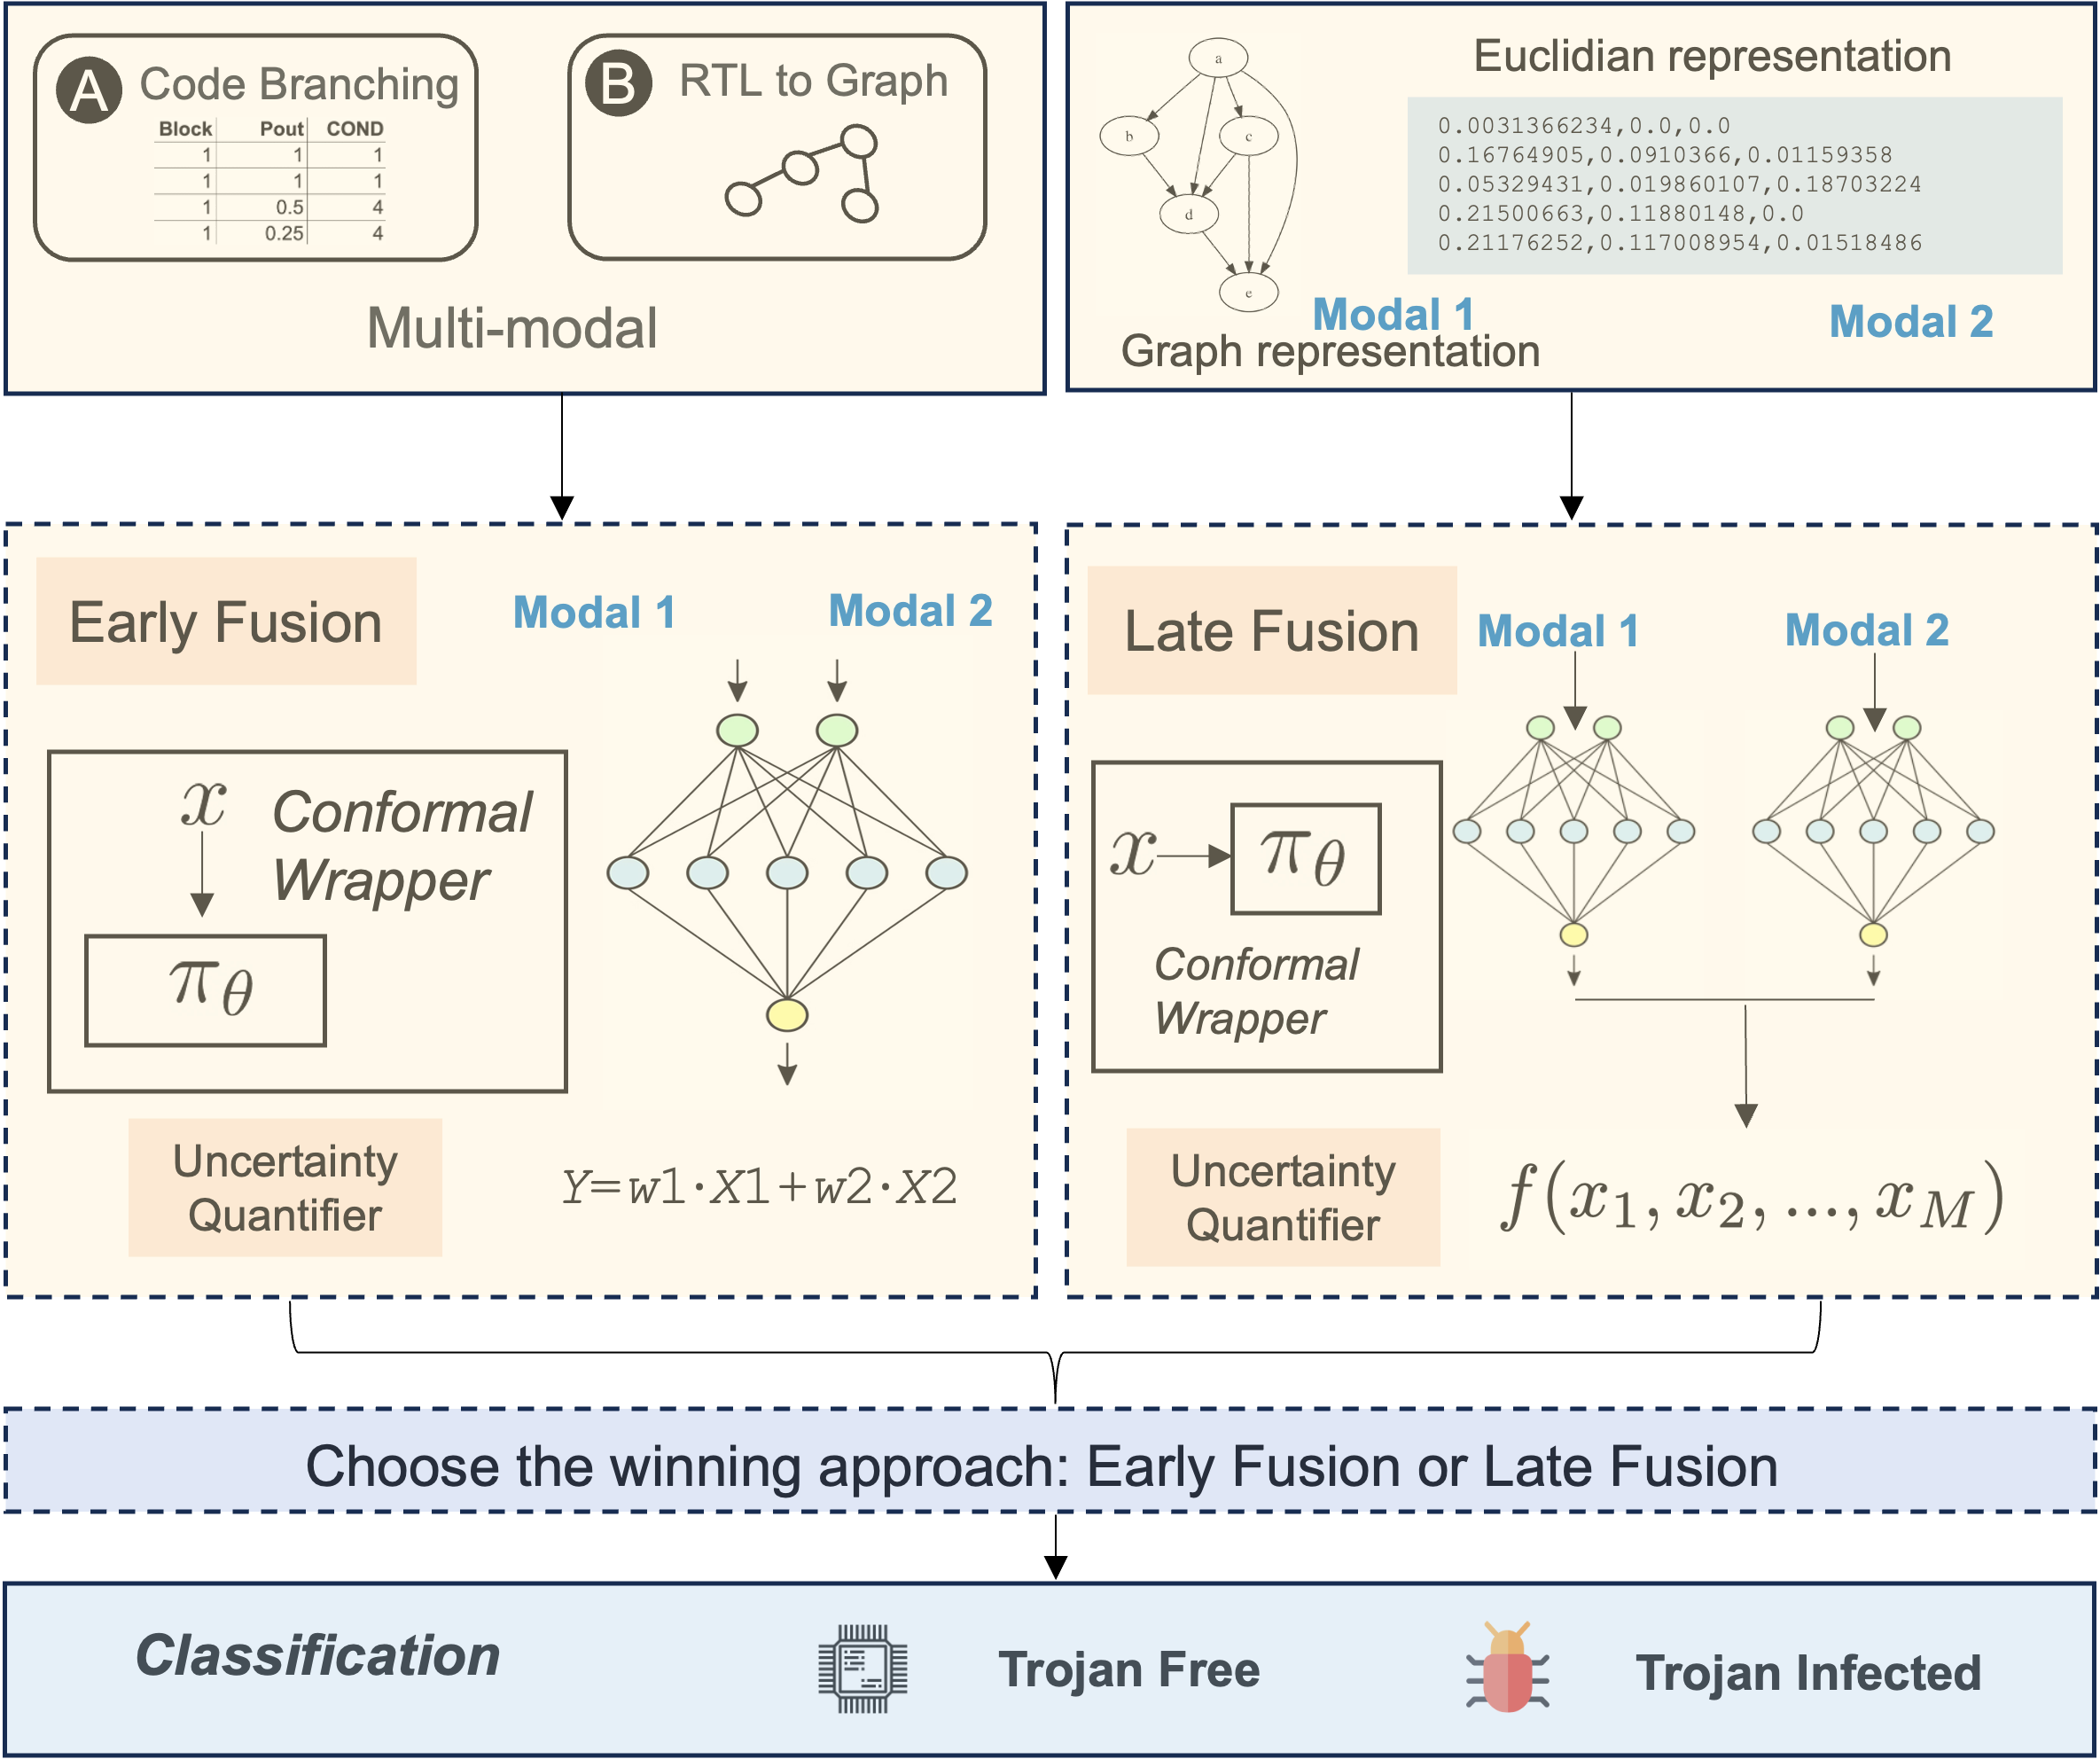
\includegraphics[width=1\textwidth]{figs/RV2.png}
   \caption{NOODLE framework: The input consists of an RTL file (Verilog), which undergoes conversion into both graph and Euclidean representations, and then input into a multimodal deep learning classifier. This classifier yields a decision indicating whether the circuit is Trojan-infected or Trojan-free.}
  \label{fig:intro}
\end{figure*}


\section*{Multimodal Hardware Trojan
Detection}
\label{sec:solution}
While state-of-the-art works on HT detection have focused mainly on choosing the right algorithm and choosing different representations of the dataset for improved accuracy, incorporating different modalities of the same data and feeding it to the ML system has not been investigated. By performing information fusion derived from different modalities, a more refined data representation can be achieved. Furthermore, in a practical scenario, we encounter missing values while collecting data, and this may lead to missing modalities when dealing with a multimodal ML approach. So, we also need a method that handles missing modalities for any given dataset. Lastly, in the domain of hardware security, it is difficult to get enough data for training, especially the labels marked as Trojan-infected because of the rarity of the event. In such a situation, we need to work with limited data.

\subsection*{Benefits of Mulitmodal Learning Approach}
The use of multimodal approach had proved better than unimodal approach based on the previous research works. 

Let, \\ 

\( X_{\text{tabular}} \) be the feature set derived from the tabular (AST) representation, \\
\( X_{\text{graph}} \) be the feature set derived from the graph (graph2vec) representation, \\
\( Y \) be the binary trojan classification (1 for Trojan Induced (TI), 0 for Trojan Free (TF)), \\
\( f_{\text{tabular}}(X_{\text{tabular}}) \) be the mapping function for the tabular representation, \\
\( f_{\text{graph}}(X_{\text{graph}}) \) be the mapping function for the graph representation, and \\
\( \theta \) be the model parameters. \\

The model can be represented as a combination of both modalities: \\

\( Y = g(f_{\text{tabular}}(X_{\text{tabular}}, \theta_{\text{tabular}}), f_{\text{graph}}(X_{\text{graph}}, \theta_{\text{graph}})) \)

In this section, the benefits are emphasized with the following points.

\begin{itemize}
    

    \item \textbf{Comprehensive information representation:} 
   \( X_{\text{combined}} = [X_{\text{tabular}}, X_{\text{graph}}] \)

    \item \textbf{Rich feature set:}
   \( X_{\text{combined}} = [X_{\text{tabular}}, X_{\text{graph}}] \)

    \item \textbf{Enhanced model robustness:}
   \( Y = g(f_{\text{tabular}}(X_{\text{tabular}}, \theta_{\text{tabular}}) \cdot f_{\text{graph}}(X_{\text{graph}}, \theta_{\text{graph}})) \)

    \item \textbf{Improved generalization:}
   \( Y = g(f_{\text{tabular}}(X_{\text{tabular}}, \theta_{\text{tabular}}) + f_{\text{graph}}(X_{\text{graph}}, \theta_{\text{graph}})) \)

    \item \textbf{Handling missing or noisy data:}
   \( Y = g(\text{impute}(f_{\text{tabular}}(X_{\text{tabular}}, \theta_{\text{tabular}})), f_{\text{graph}}(X_{\text{graph}}, \theta_{\text{graph}})) \)

\end{itemize}

\begin{algorithm}[!b]
\small
\SetKwInOut{Input}{Input}
\SetKwInOut{Output}{Output}
\Input {Number of data sources $N$; \newline
Training sets for each data source $T_1 = \{(x^{(1)}_1, y_1), \ldots, (x^{(1)}_n, y_n)\}, \ldots, T_N = \{(x^{(N)}_1, y_1), \ldots, (x^{(N)}_n, y_n)\}$, where $x^{(j)}_i$ is the $i$th data point belonging to the $j$th data source and $y_i$ is the class label of the $i$th data point; \newline
Number of classes $M$; \newline
Class labels $y^{(i)} \in Y = \{y^{(1)}, y^{(2)}, \ldots, y^{(M)}\}$; \newline
Classifiers $S_1, \ldots, S_N$ for each data source; \newline
Confidence level $E$.}

\Output {Conformal prediction regions $r_E = \{y^{(j)} : \hat{p}_j > 1 - E, y^{(j)} \in Y\}$.}

Get the new unlabeled example w.r.t each data source $x^{(1)}_{n+1}, \ldots, x^{(N)}_{n+1}$.

Evaluate conformal predictors and classifiers $S_1, \ldots, S_N$ corresponding to each data source, compute $p$-values $p^{(i)}_j$, where $i = 1, \ldots, N$ corresponds to the $i$th data source and $j = 1, \ldots, M$ corresponds to the $j$th class label.

\For {each class label $y^{(j)}$, $j = 1, \ldots, M$}{
    Compute $p$-value, $\hat{p}_j$, of combined hypothesis from $N$ modalities}

\Return $r_E$.
\caption{Uncertainty-aware information fusion}
\label{algo:mcp}
\end{algorithm}


%\section{Design Principles}
%\label{sec:desing}
\begin{algorithm}[!b]
\small
\SetKwInOut{Input}{Input}
\SetKwInOut{Output}{Output}
\Input {RTL-level files (Verliog) of circuits}
\Output {Decision (D) = Trojan-free or Trojan-infected}
\For {each circuit $C$}{
    Convert $C$ to Graph data \textbf{G} and Euclidean data \textbf{T}.
    \newline 
    \If{$\exists$ missing modalities}{
       perform GAN to impute the missing modality. 
    }
}
Feed the modalities to \textit{CNN}-based classifier.
\newline 
\For {each modalities $M$}{
    Use Algorithm \ref{algo:mcp} for uncertainty-aware information fusion.\\
    Perform early fusion.\\
    Perform late fusion. 
}
Choosing the winning fusion method.\\
\Return $D$.
\caption{Multimodal deep learning}
\label{algo:mdd}
\end{algorithm}

Our proposed \textit{NOODLE} framework is shown in Fig. \ref{fig:intro} emphasizing the design and implementation, and a pseudocode is also provided in Algorithm \ref{algo:mdd}. We choose to use two modalities, i.e., graph and tabular data representations. Methods like multimodal autoencoder \cite{jaques2017multimodal} have been used for handing missing modalities; however, we use Generative Adversarial Networks (GANs) \cite{creswell2018generative} to increase the dataset size to 500 data points as it aims to generate samples that are consistent with the joint distribution of the observed modalities and facilitate more effective multimodal fusion. The data points labeled as Trojan-Free (TF) will be segregated, and only these will be used to generate more data points using GAN so that they represent the same label, and we will do the same for data labeled as Trojan-Infected (TI). Before performing multimodal learning, we first explain the working of uncertainty-aware model fusion.

To perform an uncertainty-aware multimodal fusion, we leverage conformal prediction $p$-values for the model fusion as described in Algorithm \ref{algo:mcp}. First, we use a Convolutional Neural Network (CNN)-based classifier for graph and tabular data sources with a designed non-conformity score that provides $p$-values for each label and for each data modal. The below non-conformity score can be used in the CP framework to get calibrated conformal predictions:
\begin{equation}
NS = \sum_{t=1}^T B_t(x, y)
\end{equation}
where \(B_t(x, y)\) is the non-conformity score of \((x, y)\) computed from a classifier, \(h_t\). Thus, for every class label \(y(j)\), \(j \in \{1, ..., M\}\), we have an individual null hypothesis for each data source, \(H0_1, H0_2, ..., H0_N\), where \(M\) is the number of class labels, which in our case is either TF or TI, and \(N\) is the number of data sources. Thus, for every class label \(y(j)\), we obtain \(N\) $p$-values, \(p(i)\), \(i = 1,..., N\) (one for each modality). These $p$-values are then combined into a new test statistic \(C(p(1), ..., p(N))\), which is used to test the combined null hypothesis \(H0\) for class label \(y(j)\). 

The conformal prediction region at a specified confidence level, \(r_E\), is then presented as a set containing all the class labels with a $p$-value greater than \(1-E\). The mentioned steps helps in realization of uncertainty-aware multimodal fusion.

After obtaining a sufficient number of data points for the experiment, we implement multimodal ML using the graph and tabular data. Specifically, we have employed a CNN for binary classification. It is worth mentioning that any ML model can be optimized through hyperparameter tuning to enhance accuracy. However, our primary emphasis is on assessing the effectiveness of uncertainty-aware multimodality by accessing early and late fusions. Finally, the model will be used to make further informed decisions for the detection of HTs.


%%%%%%%%%%%%%%%%%%%%%%%%%%%%%%%%%%%%%%%%%%%%%%%%%%%%
   % Experimental results
%%%%%%%%%%%%%%%%%%%%%%%%%%%%%%%%%%%%%%%%%%%%%%%%%%%%%
\section*{Experimental results}
\label{sec:Results}
We used Python (3.9) and implemented \textit{NOODLE} on macOS (13.3.1) with 8GB RAM. The experimental results with source code and the dataset are hosted on GitHub\footnote{https://github.com/cars-lab-repo/NOODLE}.

\subsection*{Dataset}
For our experiment, we have used the features extracted from the TrustHub RTL-level (Verilog) Trojan dataset based on code branching features \cite{px6s-sm21-22} and the graph dataset in \cite{yu2021hw2vec} which includes RTL source code files (Verilog) for each IP core design containing both malicious and non-malicious functions.

{\renewcommand{\arraystretch}{1.2}%
\begin{table}[ht]
\caption{Brier score comparison for different modalities}
\centering
\begin{tabular}{lc}
\hline
\textbf{Dataset} & \textbf{Brier Score} \\ \hline 
Graph-based Data & 0.1798 \\ \hline
Tabular-based Data & 0.1913 \\ \hline
NOODLE - Early Fusion (Graph + Tabular) & 0.1685 \\ \hline
NOODLE - Late Fusion (Graph + Tabular)  & 0.1589 \\ \hline
\end{tabular}
\label{tab:table1}
\end{table}
}

\subsection*{Brier Score}
For any of the classification problem statements, the most common performance metric is model accuracy, followed by various other complementing metrics such as precision recall and F1-score. However, these metrics can be misleading in situations where the class distribution is imbalanced, as in our case. For this reason, we have used the Brier score as an evaluation metric for assessing the quality of probabilistic predictions in the classification of HTs. The Brier score, which
offers insights into accuracy and calibration, is defined as follows:
\begin{equation}
BS = \frac{1}{N} \sum_{i=1}^{N} (p_i - o_i)^2
\end{equation}
where \(N\) is the number of instances, \(p_i\) is predicted probability for instance \(i\), and \(o_i\) is the observed outcome for instance \(i\). The Brier score ranges from 0 to 1. A score of 0 indicates perfect accuracy, meaning the predicted probabilities perfectly match the actual outcomes. A score of 1 signifies complete inaccuracy, where the predicted probabilities are entirely different from the actual outcomes.

\begin{figure*}[]
\centering
  \subfloat[]
  {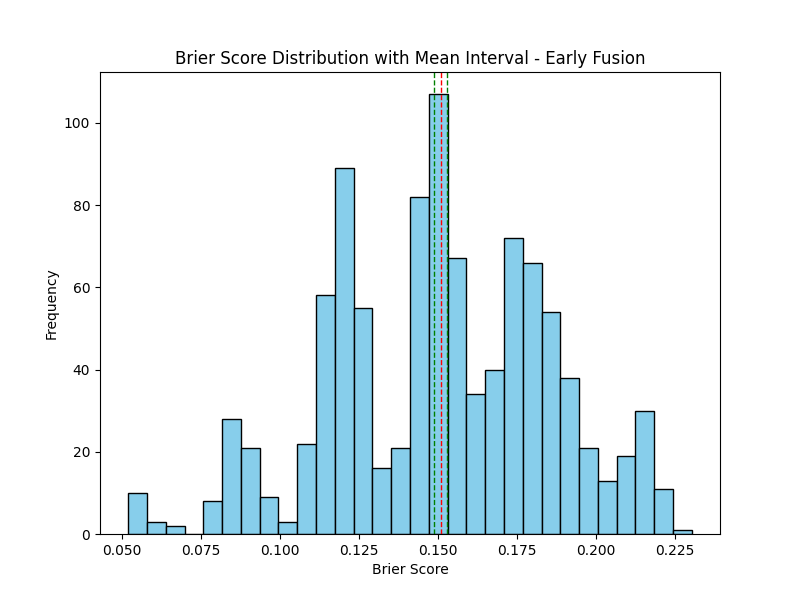
\includegraphics[width=0.5\columnwidth]{figs/early_fusion.png}}
  \subfloat[] 
  {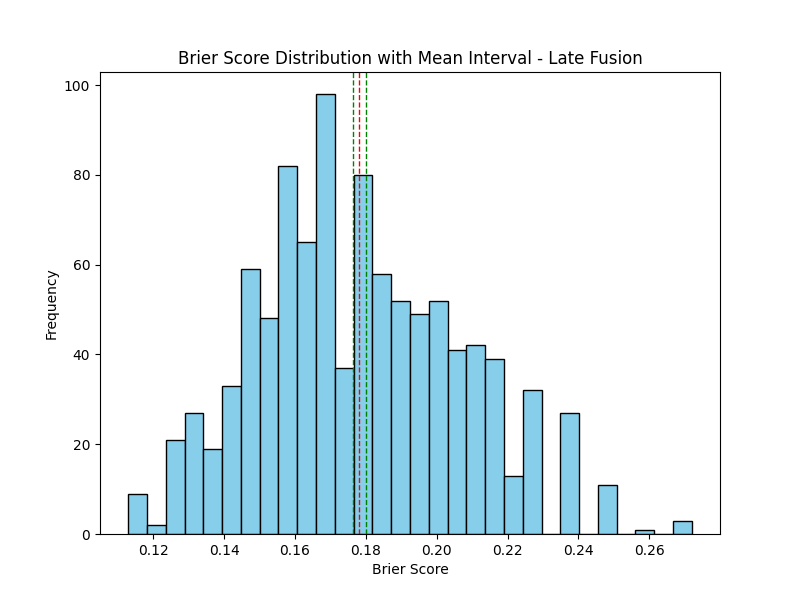
\includegraphics[width=0.5\columnwidth]{figs/late_fusion.png}}
  \caption{NOODLE's Brier score (a) Early fusion (b) Late fusion}
  \label{fig:gan}
\end{figure*}

We begin the evaluation process by independently assessing each modality. This involves conducting binary classification on both the graph dataset and the tabular data. The resulting comparative Brier scores for these classification tasks are presented in Table \ref{tab:table1}. The experimental outcome demonstrates that, when employing the same CNN-based deep learning model with identical hyperparameters, the graph dataset yields a superior Brier score (0.1798) compared to the tabular data (0.1913). It is worth noting that while we established a baseline model using CNN, any other alternative classification algorithms can also be employed in this context.

Then, we tested \textit{NOODLE} with two different information fusion approaches, i.e., early fusion (feature) and late fusion (decision). As shown in Table \ref{tab:table1}, the early fusion approach, which combines the graph and tabular data before processing, yields a Brier score of 0.1685. On the other hand, the late fusion strategy, which integrates the graph and table data after individual processing, demonstrated the best performance with a Brier score of 0.1589.

It is worth noting that neither of these data fusion methods can be deterministically labeled as superior \cite{gallo2017multimodal} as each one of them will demonstrate their potential to produce favorable outcomes when the data distribution changes. For this reason, we implemented both of the fusion approaches and chose the approach that provides a better Brier score (i.e., closer to 0), as mentioned in Step 8 of Algorithm \ref{algo:mdd}. The corresponding Brier score distribution with mean interval is also shown in Fig. \ref{fig:gan}a and Fig. \ref{fig:gan}b for early and late fusion, respectively. This provides a comprehensive view of predictive accuracy across multiple scenarios and is also useful for comparing models and understanding the variability in performance.

\subsection*{Confidence Calibration Curve}
The confidence calibration curve plots observed probabilities of occurrence as a function of the predicted probabilities for the classification model, as shown in Fig. \ref{fig:ccc}. For the model to be perfectly calibrated, it will have all data points along the diagonal; however, in our case, the model is not well calibrated because of the highly imbalanced dataset. These are the cases on which any decision-maker should focus while making a risk-aware decision and not completely relying on accuracy alone. It helps evaluate the alignment between a model's predicted probabilities and the actual likelihood of events.

A histogram at the bottom of Fig. \ref{fig:ccc} shows the predicted chance for 109 test data. It describes the distribution of the forecasts and helps with visualization of the sharpness, i.e., tendency of the predictions to lie at the extremes of the 0-1 distribution, and is equal to the variance of the predictions.

\subsection*{ROC-AUC Curve}
The Receiver Operating Characteristic (ROC) curve illustrates the balance between sensitivity and specificity in a model. It provides a visual representation of how these two metrics change as the threshold for classifying a condition varies. The Area Under the Curve (AUC), on the other hand, quantifies the likelihood that a randomly chosen pair of circuits, one with the Trojan and one without, will be accurately classified by the model. The \textit{NOODLE}'s ROC-AUC curve is given in Fig. \ref{fig:gan5}.

\begin{figure*}[]
\centering
\begin{minipage}{0.30\textwidth}
\centering
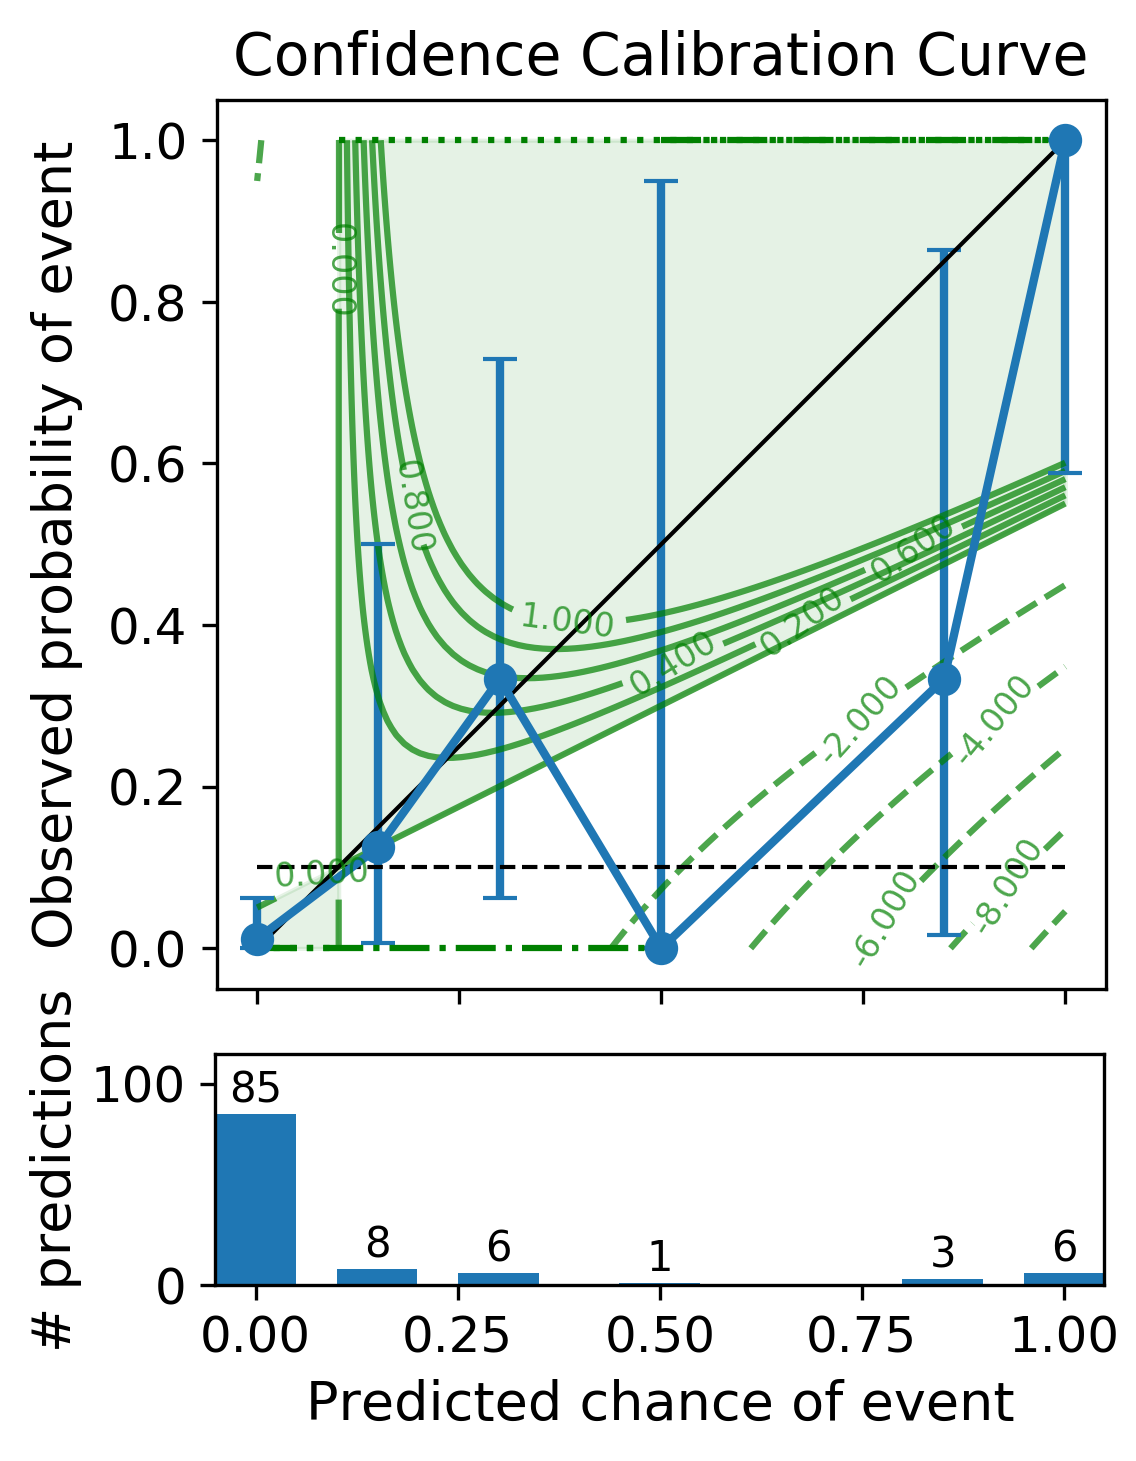
\includegraphics[width=0.79\textwidth] {figs/1.png}
\captionof{figure}{NOODLE's confidence calibration curve}
\label{fig:ccc}
\end{minipage}% 
\hspace{0.5em}
\begin{minipage}{0.30\textwidth}
\centering
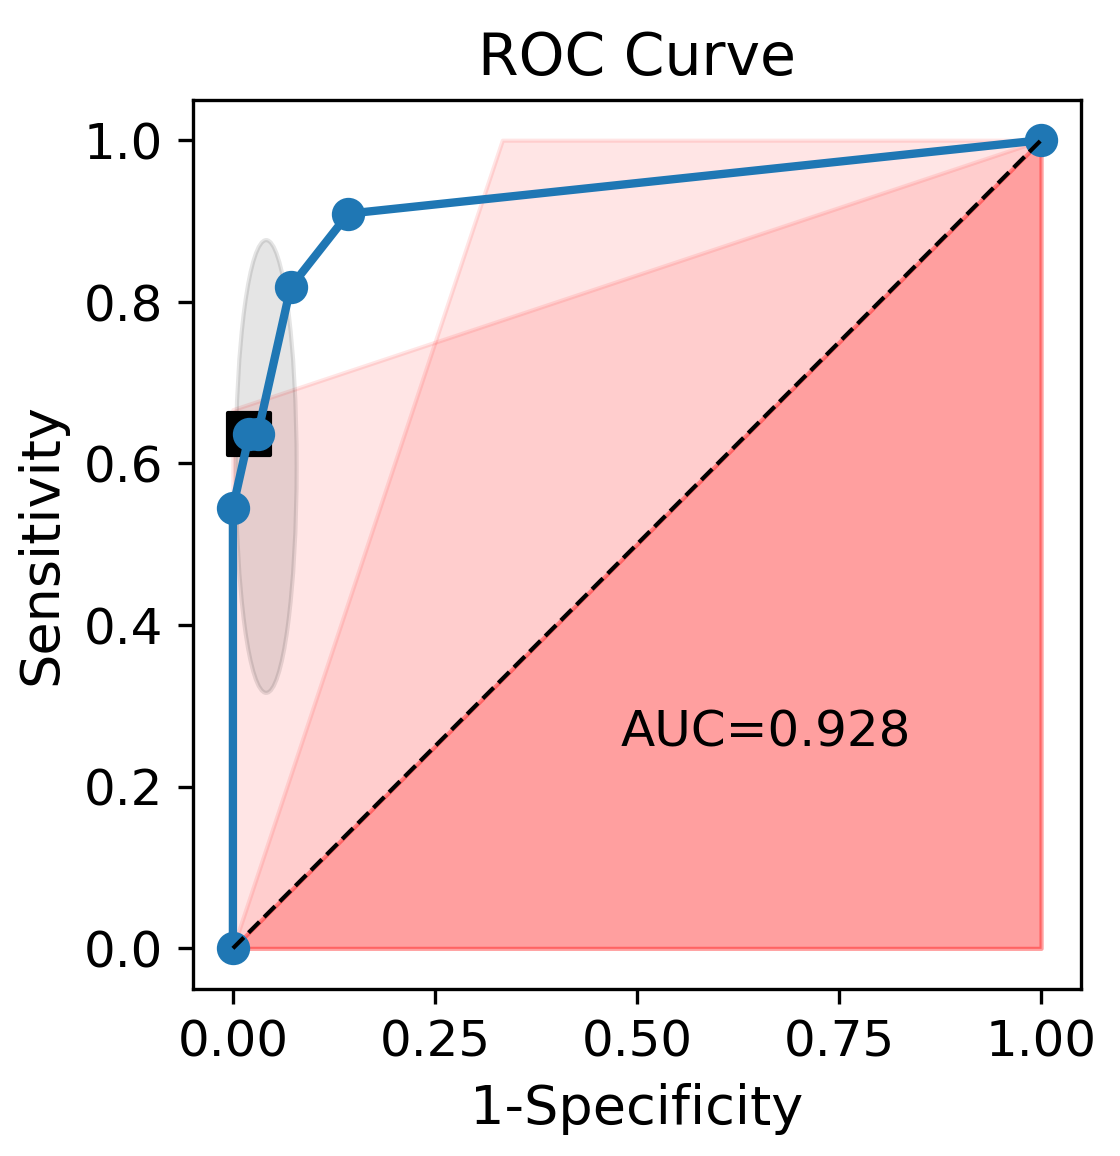
\includegraphics[width=0.98\textwidth]{figs/2.png}
\captionof{figure}{NOODLE's ROC-AUC curve under late fusion}
\label{fig:gan5}
\end{minipage}
\hspace{0.5em}
\begin{minipage}{0.35\textwidth}
\centering
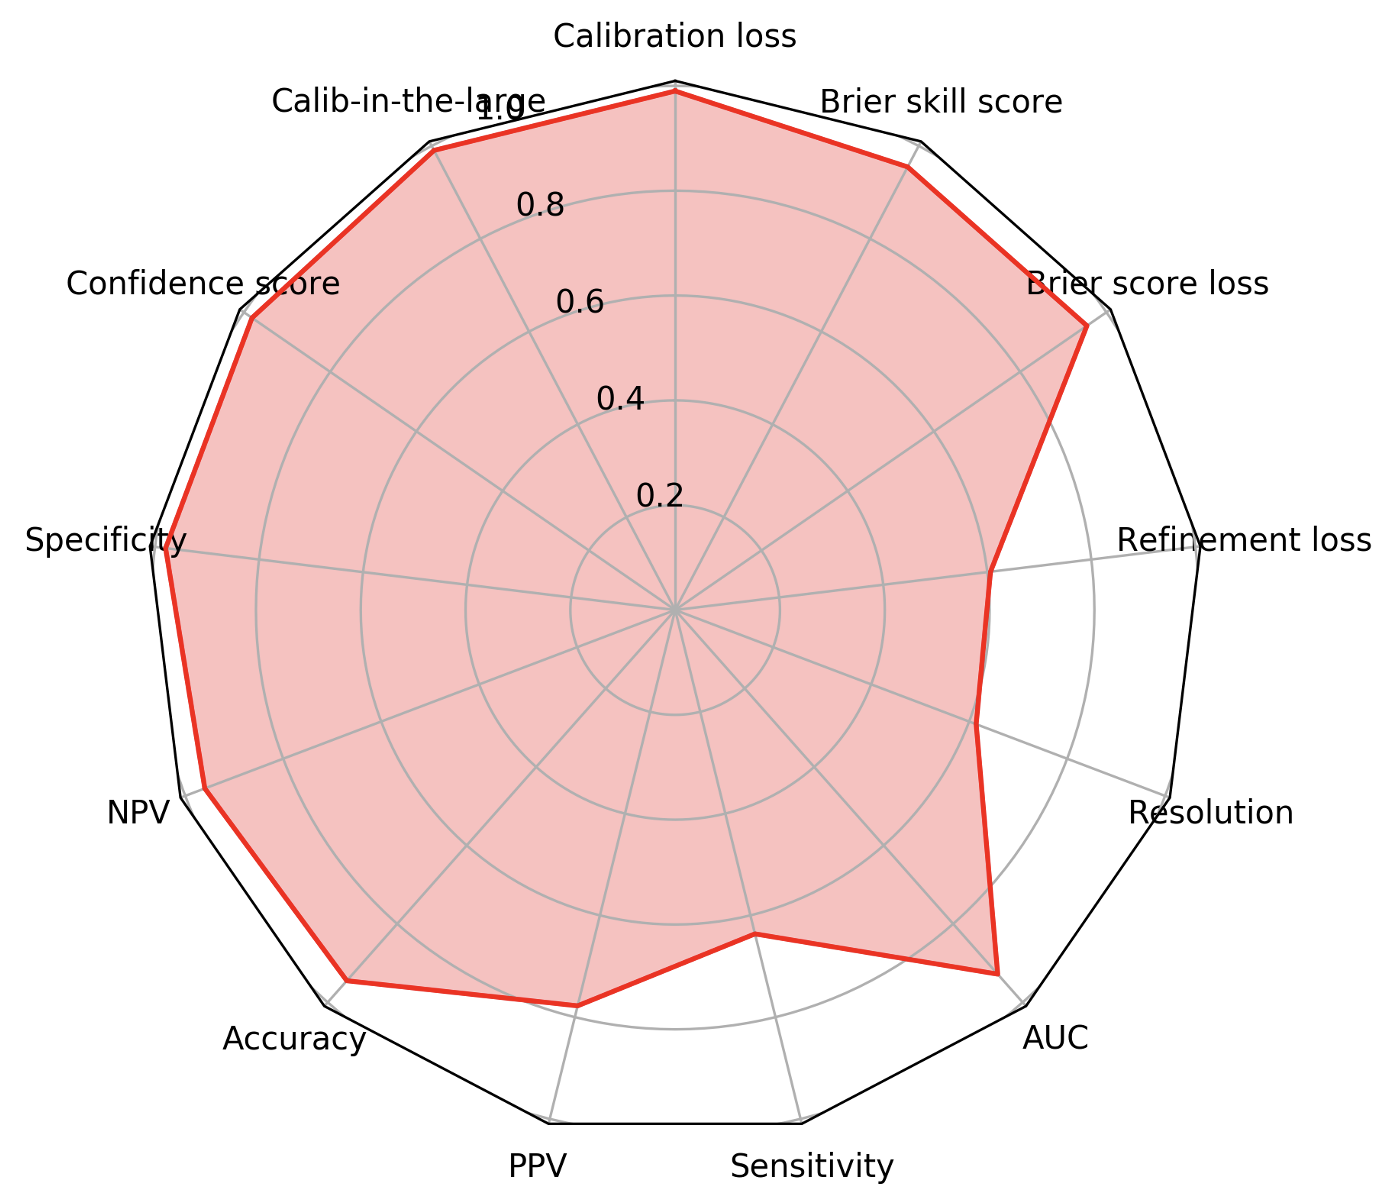
\includegraphics[width=\textwidth]{figs/radar.png}
\captionof{figure}{NOODLE's radar plot for consolidated metrics}
\label{fig:radar}
\end{minipage}
\end{figure*}

The white area represents the optimal zone for model performance, and the lightly shaded red areas represent the zones of acceptable efficacy. The values for ROC-AUC range from 0 to 1, where values near `1' suggest that it can effectively discriminate between TF and TI cases with a high degree of confidence, and if the value is near `0', the model's performance is worse than random guessing. In our case, the value is 0.928, which suggests that the model is performing well.

\subsection*{Radar Plot}
The radar plot provides a visual means of presenting complex, multi-dimensional data, as shown in Fig. \ref{fig:radar}. When appraising the effectiveness of a predictor, there is a tendency to focus narrowly on a limited set of metrics. However, the radar plot provides a method for gaining a comprehensive understanding of performance across diverse dimensions. In a radar chart, each variable is represented along its corresponding axes (some variables have been normalized to conform to the 0-1 range of the radial axis). It is also important to organize the variables in a way that clusters connected ideas or principles. This aids in conducting a thorough evaluation of various facets of performance.

In the given radar plot, we have metrics related to discrimination, which include AUC, resolution, and refinement loss. Following these are combined metrics assessing both calibration and discrimination, namely the Brier score and Brier skill score. As shown in the figure, the model is less sensitive and has high accuracy. This implies that while the model is generally accurate in its predictions, it may not be as effective in identifying all the actual TI cases. This could be due to a higher number of false negatives, which means the model is missing some of the positive cases.

\endgroup